% Mensajes Simpliciales - Tres tipos de adyacencia
% Compilar con: pdflatex simplicial_messages.tex
\documentclass[tikz,border=10pt]{standalone}
\usepackage{tikz}
\usepackage{amsmath,amssymb}
\usetikzlibrary{arrows.meta, positioning, calc}

\definecolor{gdlblue}{RGB}{41, 98, 168}
\definecolor{gdlred}{RGB}{191, 49, 49}
\definecolor{gdlgreen}{RGB}{30, 130, 76}
\definecolor{gdlorange}{RGB}{217, 130, 30}
\definecolor{gdlpurple}{RGB}{118, 56, 138}
\definecolor{gdlgray}{RGB}{140, 140, 140}
\definecolor{gdlyellow}{RGB}{190, 140, 10}

\begin{document}
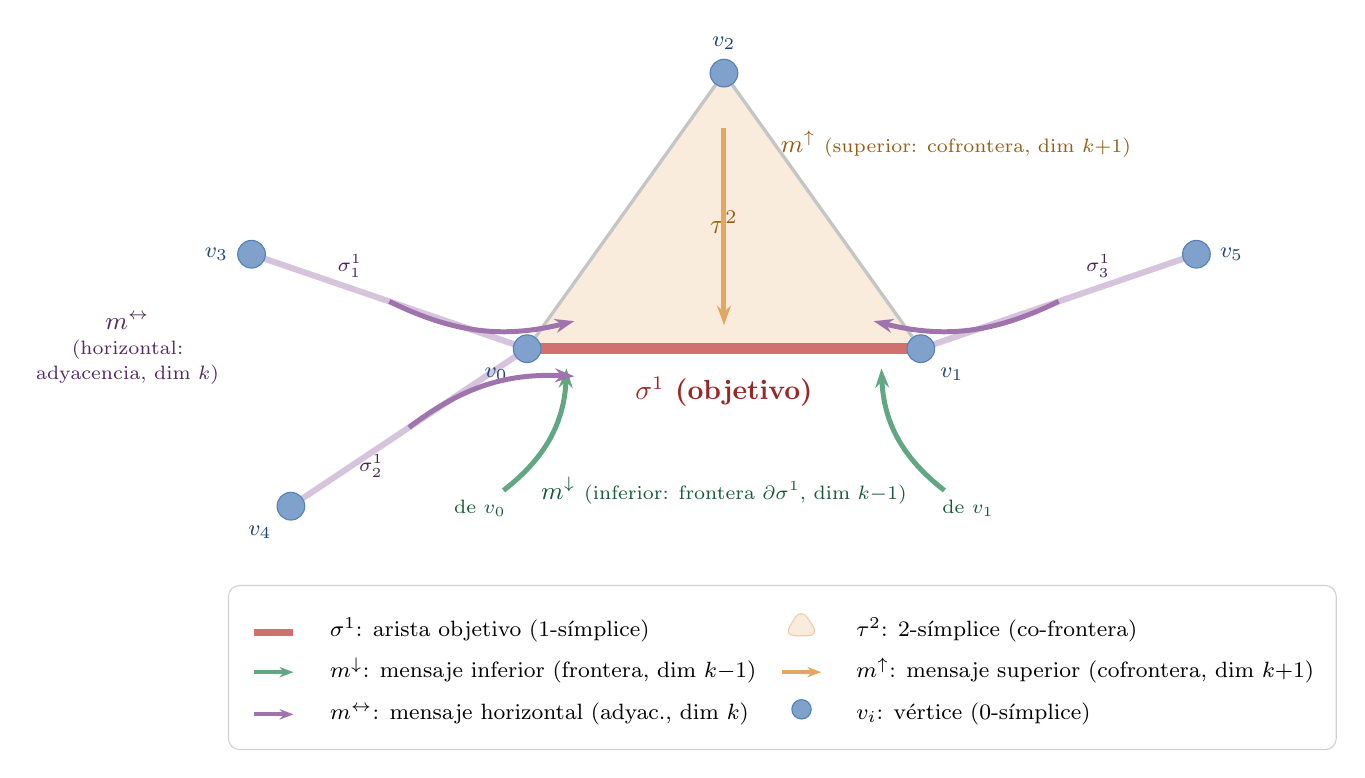
\begin{tikzpicture}[>=Stealth, font=\small,
    msg/.style={line width=1.8pt, -{Stealth[length=7pt, width=5pt]}}]

% ============================================================
% LAYOUT: Target edge is horizontal at center.
% Triangle above, adjacent edges to left and right.
% Arrows approach from 3 clear directions:
%   - Green (lower) from BELOW (vertices)
%   - Orange (upper) from ABOVE (triangle)
%   - Purple (horizontal) from LEFT and RIGHT (adjacent edges)
% ============================================================

% Target edge endpoints
\coordinate (A) at (0, 0);       % left endpoint
\coordinate (B) at (5, 0);       % right endpoint

% Triangle vertex above the target edge
\coordinate (C) at (2.5, 3.5);

% Adjacent edge endpoints (sharing one vertex with target edge)
\coordinate (D) at (-3.5, 1.2);  % connects to A (left)
\coordinate (E) at (-3.0, -2.0); % connects to A (below-left)
\coordinate (F) at (8.5, 1.2);   % connects to B (right)

% ============================================================
% 2-SIMPLEX: filled triangle A-B-C (background)
% ============================================================
\fill[gdlorange!15] (A) -- (B) -- (C) -- cycle;
\draw[gdlorange!40, line width=0.8pt] (A) -- (B) -- (C) -- cycle;

% Triangle label
\node[gdlorange!70!black, font=\normalsize] at (2.5, 1.6) {$\tau^2$};

% ============================================================
% NON-TARGET EDGES of the triangle (thin gray)
% ============================================================
\draw[gdlgray!50, line width=1.2pt] (A) -- (C);
\draw[gdlgray!50, line width=1.2pt] (B) -- (C);

% ============================================================
% ADJACENT EDGES (purple-tinted, for horizontal messages)
% ============================================================
\draw[gdlpurple!30, line width=2.2pt] (A) -- (D);
\draw[gdlpurple!30, line width=2.2pt] (A) -- (E);
\draw[gdlpurple!30, line width=2.2pt] (B) -- (F);

% Adjacent edge labels
\node[gdlpurple!60!black, font=\scriptsize, anchor=south east]
  at ($(A)!0.55!(D) + (-0.05, 0.12)$) {$\sigma^1_1$};
\node[gdlpurple!60!black, font=\scriptsize, anchor=north east]
  at ($(A)!0.55!(E) + (-0.05, -0.12)$) {$\sigma^1_2$};
\node[gdlpurple!60!black, font=\scriptsize, anchor=south west]
  at ($(B)!0.55!(F) + (0.05, 0.12)$) {$\sigma^1_3$};

% ============================================================
% TARGET EDGE — thick red, horizontal
% ============================================================
\draw[gdlred!70, line width=4pt] (A) -- (B);

% Target edge label (centered below)
\node[gdlred!80!black, font=\bfseries]
  at (2.5, -0.55) {$\sigma^1$ (objetivo)};

% ============================================================
% VERTICES (blue circles, on top of edges)
% ============================================================
\foreach \v/\lab/\pos in {
  A/$v_0$/below left,
  B/$v_1$/below right,
  C/$v_2$/above,
  D/$v_3$/left,
  E/$v_4$/below left,
  F/$v_5$/right} {
  \fill[gdlblue!60] (\v) circle (5pt);
  \draw[gdlblue!80] (\v) circle (5pt);
  \node[font=\footnotesize, gdlblue!70!black, \pos=5pt] at (\v) {\lab};
}

% ============================================================
% 1. LOWER MESSAGES (green): from boundary vertices → target edge
%    ∂(σ¹) = {v_0, v_1}: the 0-simplices bounding the target
%    Arrows come from BELOW, curving up to the edge
% ============================================================

% From v_0 (vertex A) — arrow from below-left up to left part of edge
\draw[msg, gdlgreen!70]
  ($(A) + (-0.3, -1.8)$) to[bend right=25] ($(A) + (0.5, -0.25)$);
\node[gdlgreen!70!black, font=\scriptsize, anchor=north]
  at ($(A) + (-0.6, -1.8)$) {de $v_0$};

% From v_1 (vertex B) — arrow from below-right up to right part of edge
\draw[msg, gdlgreen!70]
  ($(B) + (0.3, -1.8)$) to[bend left=25] ($(B) + (-0.5, -0.25)$);
\node[gdlgreen!70!black, font=\scriptsize, anchor=north]
  at ($(B) + (0.6, -1.8)$) {de $v_1$};

% Green label
\node[gdlgreen!70!black, font=\small, align=center,
      fill=white, fill opacity=0.8, text opacity=1,
      inner sep=3pt, rounded corners=2pt]
  at (2.5, -1.8) {$m^{\downarrow}$ \textnormal{\scriptsize(inferior: frontera $\partial\sigma^1$, dim $k{-}1$)}};

% ============================================================
% 2. UPPER MESSAGE (orange): from co-boundary triangle → target edge
%    The 2-simplex τ² containing σ¹
%    Arrow comes from ABOVE, down to the edge
% ============================================================

\draw[msg, gdlorange!70]
  (2.5, 2.8) to[bend right=0] (2.5, 0.3);

% Orange label
\node[gdlorange!70!black, font=\small, align=center, anchor=south west]
  at (3.1, 2.3) {$m^{\uparrow}$ \textnormal{\scriptsize(superior: cofrontera, dim $k{+}1$)}};

% ============================================================
% 3. HORIZONTAL MESSAGES (purple): from adjacent edges → target edge
%    Edges sharing a vertex with σ¹ (same dimension k=1)
%    Arrows come from LEFT and RIGHT
% ============================================================

% From σ¹_1 (edge A-D, shares vertex A) — arrow from left
\coordinate (m1) at ($(A)!0.5!(D)$);
\draw[msg, gdlpurple!70]
  (m1) to[bend right=20] ($(A) + (0.6, 0.35)$);

% From σ¹_2 (edge A-E, shares vertex A) — arrow from below-left
\coordinate (m2) at ($(A)!0.5!(E)$);
\draw[msg, gdlpurple!70]
  (m2) to[bend left=20] ($(A) + (0.6, -0.35)$);

% From σ¹_3 (edge B-F, shares vertex B) — arrow from right
\coordinate (m3) at ($(B)!0.5!(F)$);
\draw[msg, gdlpurple!70]
  (m3) to[bend left=20] ($(B) + (-0.6, 0.35)$);

% Purple label (left side)
\node[gdlpurple!70!black, font=\small, align=center, anchor=east,
      fill=white, fill opacity=0.8, text opacity=1,
      inner sep=3pt, rounded corners=2pt]
  at (-3.8, 0.0) {$m^{\leftrightarrow}$\\[-2pt]\textnormal{\scriptsize(horizontal:}\\[-2pt]\textnormal{\scriptsize adyacencia, dim $k$)}};

% ============================================================
% LEGEND BOX
% ============================================================
\node[anchor=north west, draw=gdlgray!40, rounded corners=4pt,
      fill=white, fill opacity=0.95, text opacity=1,
      inner sep=8pt, font=\footnotesize]
  at (-3.8, -3.0) {%
    \begin{tabular}{@{}cl@{\quad}cl@{}}
      \tikz\draw[gdlred!70, line width=2.5pt] (0,0) -- (0.5,0); &
      $\sigma^1$: arista objetivo (1-s\'{i}mplice) &
      \tikz\fill[gdlorange!15, draw=gdlorange!40]
        (0,0) -- (0.45,0) -- (0.22,0.35) -- cycle; &
      $\tau^2$: 2-s\'{i}mplice (co-frontera) \\[5pt]
      %
      \tikz\draw[-{Stealth[length=5pt]}, gdlgreen!70, line width=1.5pt]
        (0,0.1) -- (0.5,0.1); &
      $m^{\downarrow}$: mensaje inferior (frontera, dim $k{-}1$) &
      \tikz\draw[-{Stealth[length=5pt]}, gdlorange!70, line width=1.5pt]
        (0,0.1) -- (0.5,0.1); &
      $m^{\uparrow}$: mensaje superior (cofrontera, dim $k{+}1$) \\[5pt]
      %
      \tikz\draw[-{Stealth[length=5pt]}, gdlpurple!70, line width=1.5pt]
        (0,0.1) -- (0.5,0.1); &
      $m^{\leftrightarrow}$: mensaje horizontal (adyac., dim $k$) &
      \tikz\fill[gdlblue!60, draw=gdlblue!80] (0.15,0.1) circle (3.5pt); &
      $v_i$: v\'{e}rtice (0-s\'{i}mplice) \\
    \end{tabular}%
  };

\end{tikzpicture}
\end{document}
